\startchapter{Approach and Solution to Real Problem}
\label{chapter:Simplified molecular model}

\section{Description}
\section{}
\section{Linear Programming Model}
\subsection{Advantages of Linear Programming}
Introduce the simplex method, the toolkit.
Linear programming can deal with thousands of variables.\\

Linear programming is a convex, deterministic process, and it is guaranteed to converge to a single global optimal if there is a solution space. Linear Programming problems are intrinsically easier to solve than general nonlinear problems.\\

For a linear programming problem, it is by nature that there are three kinds of situations may happen.\\

First, there is no feasible solution.\\

Second, there are feasible solutions, and the solutions space is bounded in a polyhedron, and only one globally optimal solution(either a single point or multiple equivalent points along a line) exists. Furthermore, in this unique and convex feasible region, the optimal solution is at one of the vertex of this convex polygon.\\

Third, the solution space is unbounded, there are multiple solutions, however, no optimal solution for the existing problem.\\

Because of this property, it is guaranteed that if linear programming solver returns a solution, then this solution is the global optimal one for the problem.\\

Simplex method:
Introduce Linear Programming solver:


	
	
	

	
	
	
	
	
	
Compare linear programming with quadratic programming, why linear programming is a better 	 	approach to the problem? (Having problems finding related work or how to prove it myself)
	
	Is there only computational gain?
	Also consider the model itself and solution space	
(The problem is defined as "Candidate ratio problem" in Kai's thesis, same here???)
	to determine the level of similarity between spectra is not an easy task 
	
	How should I introduce Linear Programming here?
	The advantages of linear programming are: 
	
\subsection{Linear Programming Model for Toy Spectroscopy Model}
Before working on a real molecule, we set up a toy spectroscopy model to better understand Linear Programming and spectroscopy techniques. In this toy model, we use the following equation to generate the spectroscopy, 
\begin{eqnarray}
& f_{\theta}(x) = \displaystyle\sum^{4}_{q=1} A_q^2 * cos^2(\theta - \theta_q)\frac{\gamma^2}{(x- w_q)^2 + \gamma^2} \nonumber \\
& A:~amplitude \nonumber \\
& \theta_q : angle \nonumber \\
& \gamma: width \nonumber \\
& w_q : frequency \nonumber 
\end{eqnarray}

What's more, this molecule only contains 4 vibration modes, with the peaks happen at frequency of 2850, 2960, 3050 and 3200, and the widths for the peaks are 5, 10, 5 and 15, and the heights, which are 1, 0.7, -0.2 and 0.5 respectively. The comparing angle for each peak( What does those angle refer???) is 15, 90, 0 and 60. We generate 10 candidate spectra with 10 different $\theta$ values:
$\theta = 0^{\circ}, 10^{\circ}, 20^{\circ}, 30^{\circ}, 40^{\circ}, 50^{\circ}, 60^{\circ}, 70^{\circ}, 80^{\circ}, 90^{\circ} $ \\

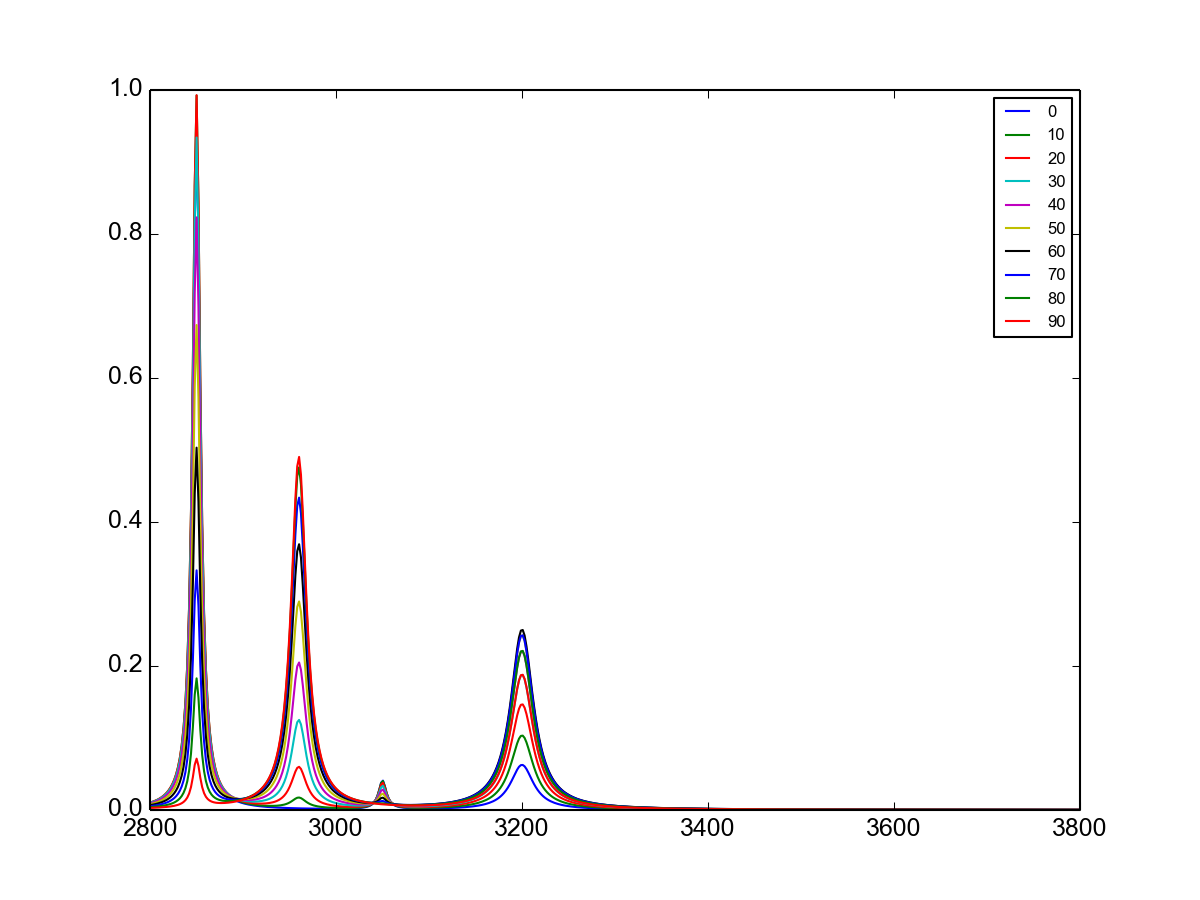
\includegraphics[scale=1,bb=0 0 30 30]{LP1.png}

As you can see from the graph that, these 10 candidates have peaks at the same frequency. And the only difference on $\theta$ makes them very similar to each other. This also makes it really difficult to obtain exact composition for the targeted spectrum, as various combinations of candidates are possible to achieve the targeted spectrum.

As an example, we compose a target spectrum by combining 15 percent $\theta$ of 20 degree's spectrum and 85 percent of $\theta$ of 70 degree's spectrum: $0.15*f_{20}(x) + 0.85*f_{70}(x)$. \\


The linear programming model that we construct to check if the optimal solution returned actually match the known composition is as following. The model has used in the studies of \cite{03}  and \cite{04}. \\
\begin{eqnarray}
& minimize \displaystyle\sum^{points}_{p=1} \left| Target- \displaystyle\sum^{candidates}_{c=1}p_{c}f_{\theta}(x) \right| \nonumber \\
& p_c: percentage ~of~ each~ candidate \nonumber \\
& p: number~ of~ points~ selected~ both~ from~ candidates~ and~ Target \nonumber 
\end{eqnarray}
 
In this model, the unknown percentage of each candidate is the decision variable, it is denoted by $p_c$. We select data points along the wavelength frequency,the data point is denoted by $p$ here. Based on each data point, we calculate the absolute residual between target spectrum and the one composed by the decision variables. Then the objective function is to minimize of the sum of the absolute residual over all the data points. \\

However, in order to actually apply Linear Programming, we need to get rid of the absolute sign in the objective function. We achieve this goal by introducing one more variable X and two more constraints for each data point. Therefore:\\

For each point:
\begin{eqnarray} 
& X = \left| Target-\displaystyle\sum^{candidates}_{c=1}p_{c}f_{\theta}(x) \right| \nonumber \\
&  X \geq Target-\displaystyle\sum^{candidates}_{c=1}p_{c}f_{\theta}(x)   \nonumber \\
& X \geq -Target+\displaystyle\sum^{candidates}_{c=1}p_{c}f_{\theta}(x)  \nonumber
\end{eqnarray} 

We then convert the previous model into one that can actually be solved by Linear Programming solver:\\

\begin{eqnarray} 
& minimize \displaystyle\sum^{points}_{p=1} X_p \nonumber \\
& X_1 - Target_1 + \displaystyle\sum^{candidates}_{c=1}p_{c}f_{\theta}(x_1) \geq 0 \nonumber \\
& X_1 + Target_1 - \displaystyle\sum^{candidates}_{c=1}p_{c}f_{\theta}(x_1) \geq 0 \nonumber \\
& ... \nonumber \\
& X_n - Target_n + \displaystyle\sum^{candidates}_{c=1}p_{c}f_{\theta}(x_n) \geq 0 \nonumber \\
& X_n + Target_n - \displaystyle\sum^{candidates}_{c=1}p_{c}f_{\theta}(x_n) \geq 0 \nonumber \\
& \displaystyle\sum^{candidates}_{c=1}p_{c} = 1 \nonumber
\end{eqnarray} 

The last equality restrict the sum of the percentage to 1.

During the try-out, we first select the data points at the peaks, which are four points at frequency of 2850, 2960, 3050 and 3200. We then construct the Linear Programming model based on these data points. The result returned by LP-solver matched to the known one. However, if we randomly select four data points, the returned result usually does not match to the know one. At the end, we increase the number of data points, at each 5 wavelength frequency gap, a data point will be selected. And the returned result will eventually match to the known one. \\

The more data points we select, the more information about the candidates and targeted spectrum we will have in our model. Therefore, the more complicated and complete model we will construct. As we select one data point, a new variable is introduced to our model, meanwhile, two new constraints are brought into our model as well. This means that solution space is further and better restricted. When we select data points only on the peaks, these data points already contains enough information for the solver to distinguish the candidates. However, if we randomly select four data points, they may not contain enough information in order to construct the model to obtain the desired result. 

  




		
\subsection{Explain any special feature that related to our problem} 
		 




%\input chapters/3/sec_latexhelp
